\documentclass[11pt]{article}

\usepackage[french]{babel}
\usepackage[utf8]{inputenc}

\usepackage[T1]{fontenc}


\usepackage{booktabs}
%% Camille, change the color as you wish
\usepackage[pdftex,dvipsnames,usenames]{xcolor}
\usepackage[pdftex,colorlinks=true,urlcolor=ForestGreen,citecolor=Blue,linkcolor=BrickRed]{hyperref} % Must be loaded before cleveref
\usepackage{paralist}


\usepackage{graphicx}
\graphicspath{{./fig}}

\newif\ifdraftmode
\draftmodetrue
% \draftmodefalse

\usepackage{amsmath,amsthm,amssymb}
\usepackage[normalem]{ulem}

\textwidth 16cm
%\textheight 22cm
\evensidemargin 0cm
\oddsidemargin 0cm

\usepackage{colors}
\usepackage{encarts}
\usepackage{tikzstyles}
\usepackage{theoremes}
\usepackage{macros}


\newcommand{\instance}[1]{instance de type #1 du tableau~\ref{tab:instances} page~\pageref{tab:instances}}
\title{Activité : Partition}
\date{}

\begin{document}

\ifdraftmode
\selectcolormodel{gray}
\fi

\maketitle
\tableofcontents

\section{Description du problème}

  \begin{definition}{Partition d'un ensemble}
    Un \emph{multiensemble} (parfois appelé sac) est un ensemble dans lequel chaque élément peut apparaître plusieurs fois.
    Soit un multiensemble $S$ de $n$ entiers naturels :

    $$S = \{s_i\ |\ s_i > 0\}_{1\leq i \leq n}.$$

    Une \emph{(bi)partition} de $S$ est constituée de deux sous-multiensembles $S_1$ et $S_2$ tels que :
    \begin{itemize}
      \item $S_1$ et $S_2$ sont non vides:  $S_1 \neq \emptyset$ et $S_2 \neq \emptyset$ ;
      \item $S_1$ et $S_2$ sont disjoints:  $S_1 \cap S_2 = \emptyset$ ;
      \item $S_1$ et $S_2$ recouvrent $S$:  $S_1 \cup S_2 = S$.
    \end{itemize}
  \end{definition}

  \begin{exemple}{Partition d'un ensemble}
    Soit un multiensemble $S = \{1,2,3,4,5\}$.
    \begin{itemize}
      \item Les multiensembles $S_1$ et $S_2$ forment une partition de $S$.
        \begin{itemize}
          \item $S_1 = \{1\}$ et $S_2 = \{2,3,4,5\}$
          \item $S_1 = \{2, 4\}$ et $S_2 = \{1,3,5\}$
        \end{itemize}
      \item Les multiensembles $S_1$ et $S_2$ ne forment pas une partition de $S$.
        \begin{itemize}
          \item $S_1 = \{1,2,3,4,5\}$ et $S_2 = \emptyset$, car $S_2$ est vide.
          \item $S_1 = \{1,2,3\}$ et $S_2 = \{3,4,5\}$, car leur intersection est non vide.
          \item $S_2 = \{1,2\}$ et $S_2 = \{4, 5\}$, car 3 est dans $S$, mais n'appartient ni à $S_1$ ni à $S_2$.
        \end{itemize}
    \end{itemize}
  \end{exemple}

  \begin{definition}{Partition parfaite d'un multiensemble pair}
    Un multiensemble d'entiers $S$ est dit \emph{pair} si la somme des entiers de $S$ est pair.

    Une \emph{partition parfaite} d'un multiensemble pair est une partition telle que la valeur absolue de la différence entre la somme des entiers de $S_1$ et la somme des entiers de $S_2$ est 0.
  \end{definition}

  \begin{exemple}{Partition parfaite d'un multiensemble pair}
    $S = \{1,2,3,4\}$ est un multiensemble pair.
    \begin{itemize}
      \item $S_1 = \{1,3\}$ et $S_2 = \{2,4\}$ ne forment pas une partition parfaite.
      \item $S_1 = \{1,4\}$ et $S_2 = \{2,3\}$ forment une partition parfaite.
    \end{itemize}
  \end{exemple}

  \begin{definition}{Partition parfaite d'un multiensemble impair}
    Un multiensemble d'entiers $S$ est dit \emph{impair} si la somme des entiers de $S$ est impair.

    Une \emph{partition parfaite} d'un multiensemble impair est une partition telle que la valeur absolue de la différence entre la somme des entiers de $S_1$ et la somme des entiers de $S_2$ est 1.
  \end{definition}

  \begin{exemple}{Partition parfaite d'un multiensemble impair}
    $S = \{1,2,3,4, 5\}$ est un multiensemble impair.

    \begin{itemize}
      \item $S_1 = \{2, 4\}$ et $S_2 = \{1,3,5\}$ ne forment pas une partition parfaite.
      \item $S_1 = \{1, 2, 5\}$ et $S_2 = \{3,4\}$ forment une partition parfaite.
    \end{itemize}
  \end{exemple}

  \begin{definition}{Problème de partitionnement}
  En informatique, le problème de partitionnement consiste à déterminer si une partition parfaite d'un ensembles d'entiers existe. C'est un problème \emph{NP-complet}. Cependant, il existe plusieurs algorithmes qui résolvent efficacement le problème que ce soit de manière approchée ou optimale. Pour ces raisons, il est réputé ``le plus facile des problèmes difficiles" \cite{Mertens2003}.
\end{definition}
  % Le problème de partitionnement se décline aussi en problème d'optimisation dans lequel on recherche une partition minimisant la valeur absolue de la différence entre la somme des entiers des deux sous-ensembles de la partition.
  % Ce problème d'optimisation est \emph{NP-difficile}.


\section{Partition parfaite des entiers de 1 à $n$}

  \begin{exercice}{}
    Trouver une partition parfaite des entiers de 1 à $n$ pour $n =4, 5, 6, 7, 8$.
  \end{exercice}


  \begin{figure}[htbp]
    \centering
    \resizebox{0.6\linewidth}{!}{
      
\begin{tikzpicture}
  \pic at (0, -16) {subset sum = {capacity = 5, sizes = {1,4,2,3}, deck = {1,1,0,0}}};
  \pic at (0, -20) {subset sum = {capacity = 7, sizes = {1,2,5,3,4}, deck = {2,1,1,0,0}}};
  \pic at (0, -24) {subset sum = {capacity = 10, sizes = {1,2,3,6,4,5}, deck = {1,2,1,1,0,0}}};
  \pic at (0, -28) {subset sum = {capacity = 14, sizes = {1,2,3,4,7,5,6}, deck = {1,1,2,1,1,0,0}}};
  \pic at (0, -32) {subset sum = {capacity = 18, sizes = {1,8,2,7,3,6,4,5}, deck = {1,1,1,1,0,0,0,0}}};
\end{tikzpicture}
    }
    % 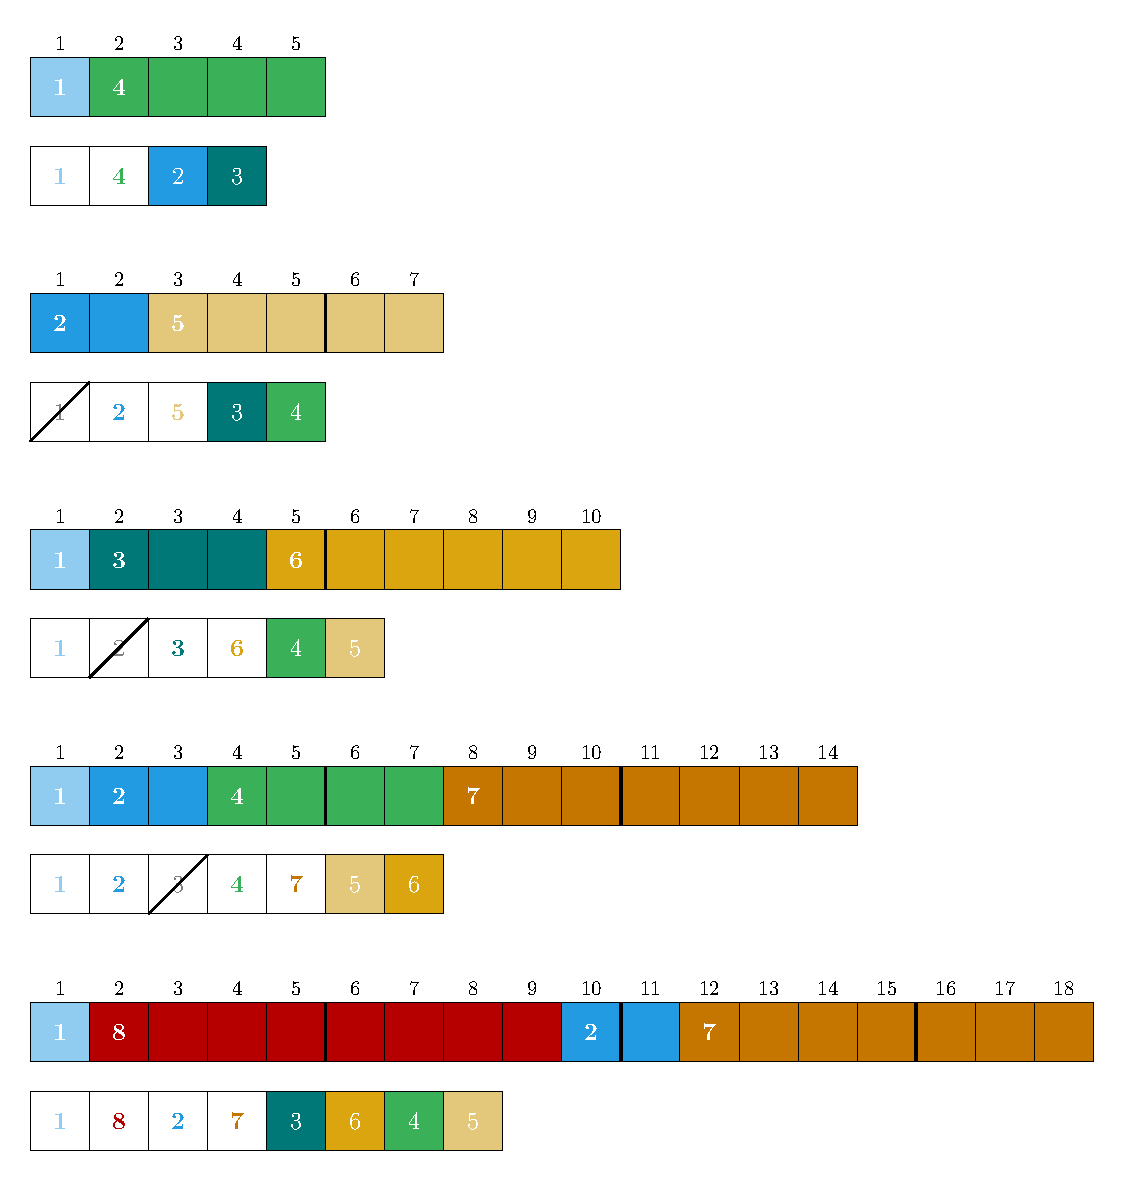
\includegraphics[width=0.6\linewidth]{partition-8.pdf}
    \caption{Partition parfaite des entiers de 1 à $n$.}
  \end{figure}


  \begin{definition}{Algorithme}
    Un \emph{algorithme} répond à un problème. Il est composé d’un ensemble d’étapes simples nécessaires à la résolution, dont le nombre varie en fonction de la taille des données.
  \end{definition}

  \begin{remarque}{}
    Plusieurs algorithmes peuvent répondre à un même problème.
  \end{remarque}

  \begin{remarque}{}
    Un algorithme peut répondre à plusieurs problèmes.
  \end{remarque}

  \begin{exercice}{}
    Donner un algorithme pour trouver une partition parfaite des entiers de 1 à $n$.
  \end{exercice}

  \begin{indice}
    Distinguer les cas en fonction du reste $r$ de la division euclidienne de $n$ par 4. C'est-à-dire qu'il existe $k \geq 0$ et $0 \leq r \leq 3$ tels quel $n = 4 \times k + r$.
    % \begin{tabular}{|*{5}{c |}}
    %   \hline
    %   1 & 2 & $\cdots$ & $p-1$ & $p$\\
    %   $2p$ & $2p-1$ & $\cdots$ & $p+2$ & $p+1$\\\hline
    % \end{tabular}
    % Que remarquez-vous pour chacune des colonnes de ce tableau ?
  \end{indice}


  \begin{algorithme}{Partition parfaite des entiers de 1 à $n$.}
    \begin{itemize}
    \item Soit $n = 4 \times k + r$ le quotient $k$ et le reste $r$ ($0 \leq r \leq 3$) de la division euclidienne de $n$ par 4.
      \begin{itemize}
      \item Si $r=1$, alors éliminer l'objet 1.
      \item Si $r=2$, alors ranger l'objet 1 et éliminer l'objet 2.
      \item Si $r=3$, alors ranger les objets 1 et 2 et éliminer l'objet 3.
      \end{itemize}
  \item Répéter $2 \times k$ fois l'action suivante \\ (ou de manière équivalente, répéter tant que le sac n'est pas rempli) :
    \begin{itemize}
    \item ranger le plus petit et le plus grand objet.
    \end{itemize}
  \end{itemize}
  \end{algorithme}

\begin{remarque}{}
    Ce problème admet une symétrie évidente puisque l'on peut inverser la partition, c'est-à-dire échanger les ensembles $S_1$ et $S_2$.
    De manière générale, on peut toujours échanger des objets entre $S_1$ et $S_2$ si cela ne change pas leurs sommes.
  \end{remarque}


\begin{exercice}{}
  \begin{itemize}
  \item Trouver une partition parfaite des entiers de 1 à 16.
  \item Remarquez que toutes les paires d'objets formées par l'algorithme ont la même somme.
    Trouvez d'autres partitions parfaites par échanges successifs.
  \end{itemize}

\end{exercice}


\begin{table}[htbp]
  \centering
      \begin{tabular}{llll}
      \toprule
      Type & Niveau & Sac & Capacité \\
      \midrule
             & Facile & 11, 8, 7, 5, 2, 1 & 17 \\
      1 & Intermédiaire & 16, 12, 10, 9, 6, 5, 3, 2, 1 & 32 \\
             & Difficile & 16, 15, 13, 12, 9, 8, 6, 5, 4, 3, 2, 1 & 47 \\
      \midrule
             & Facile & 14, 13, 11, 7, 5, 3 & 26 \\
      2 & Intermédiaire & 16, 15, 14, 13, 12, 9, 8, 6, 1 & 47 \\
             & Difficile & 16, 15, 13, 12, 11, 10, 8, 7, 6, 4, 3, 2 & 53 \\
      \midrule
             & Facile & 13, 11, 9, 8, 6, 4 & 25 \\
      3 & Intermédiaire & 16, 15, 14, 10, 9, 8, 6, 5, 3 & 43 \\
             & Difficile & 16, 15, 14, 13, 12, 11, 10, 8, 7, 6, 4, 3 & 59 \\
      \midrule
             & Facile & 16, 15, 11, 4, 2, 1 & 24 \\
      4 & Intermédiaire & 18, 15, 13, 10, 8, 5, 3, 2 & 37 \\
             & Difficile & 18, 17, 16, 15, 14, 5, 2, 1 & 44 \\
      \bottomrule
      \end{tabular}
  \caption{Instances du problème de partitionnement.}
  \label{tab:instances}
\end{table}

    \section{Algorithmes gloutons}

  \begin{definition}{Algorithme glouton}
    Un \emph{algorithme glouton} est un algorithme qui suit le principe de faire, étape par étape, un choix optimum local.
    Dans certains cas, cette approche aboutit à un optimum global, mais dans le cas général c'est une heuristique qui n'aboutit pas nécessairement à un optimum global.
  \end{definition}


  \begin{algorithme}{Algorithme glouton}
    \label{algo:gs}
    \begin{itemize}
    \item Déterminer la capacité du sac : la somme des objets divisée par deux.
    \item Trier les objets par ordre décroissant.
    \item  Répéter tant qu'il reste des objets et que le sac n'est pas rempli :
      \begin{itemize}
      \item ranger le plus grand objet dans le sac si la capacité le permet.
      \item Sinon éliminer l'objet.
      \end{itemize}
  \end{itemize}
  \end{algorithme}



  \begin{exercice}{}
    Appliquer l'algorithme glouton sur une \instance{1}.
  \end{exercice}

  \begin{figure}[htbp]
    \centering
    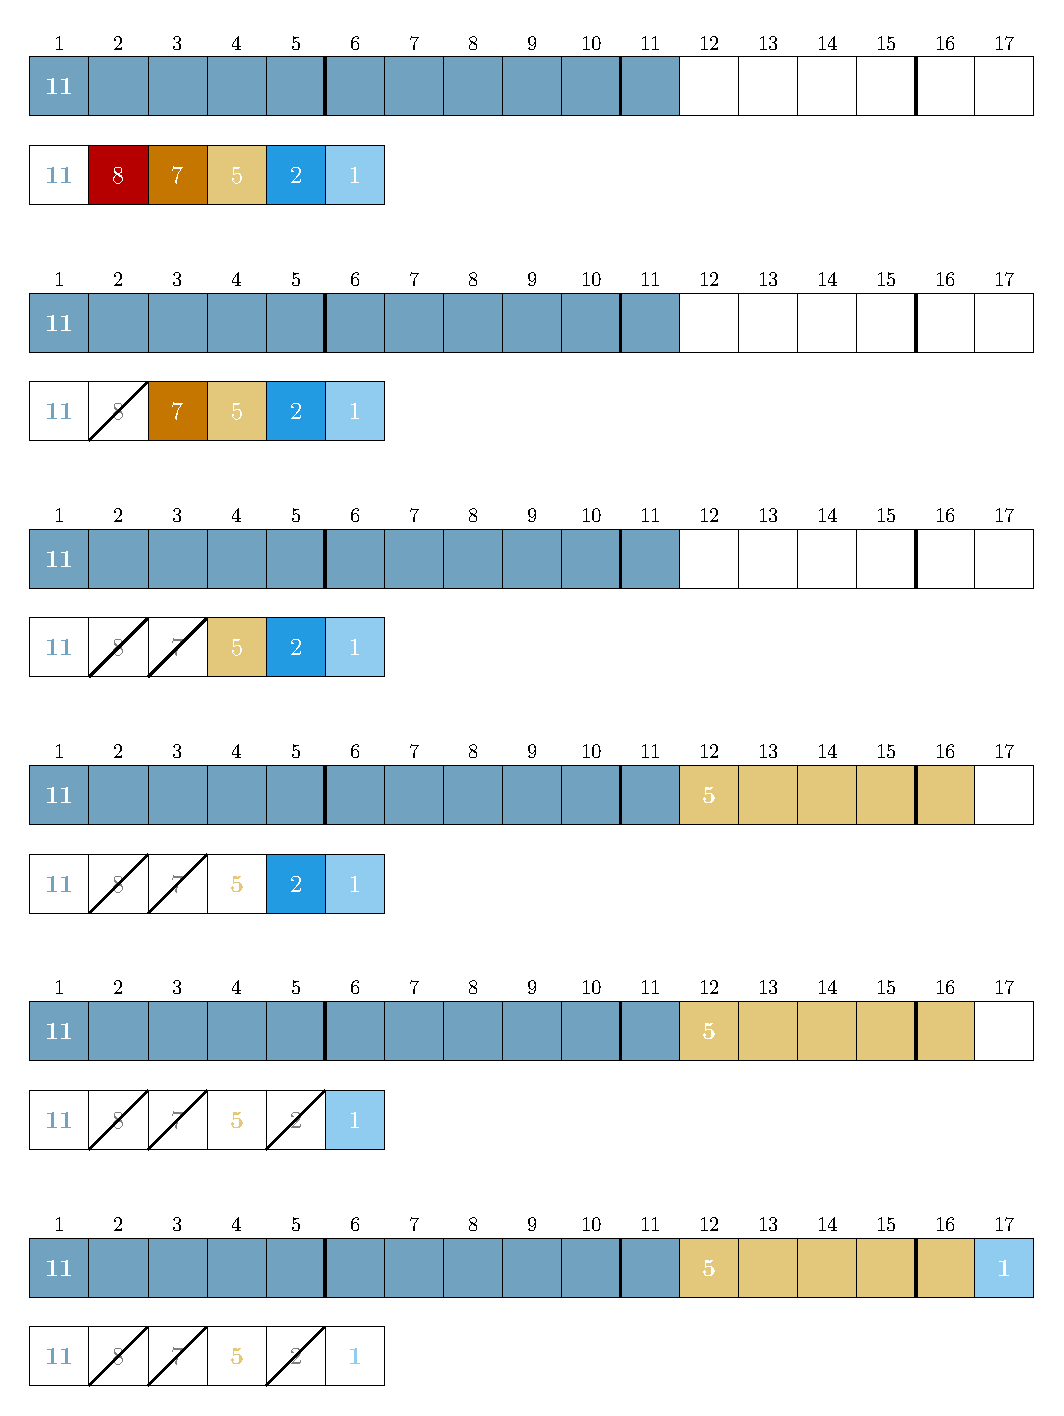
\includegraphics[width=0.6\linewidth]{ex1-6-GS.pdf}
    \caption{Solution de l'instance facile de de type 1.}
  \end{figure}

    \begin{figure}[htbp]
    \centering
    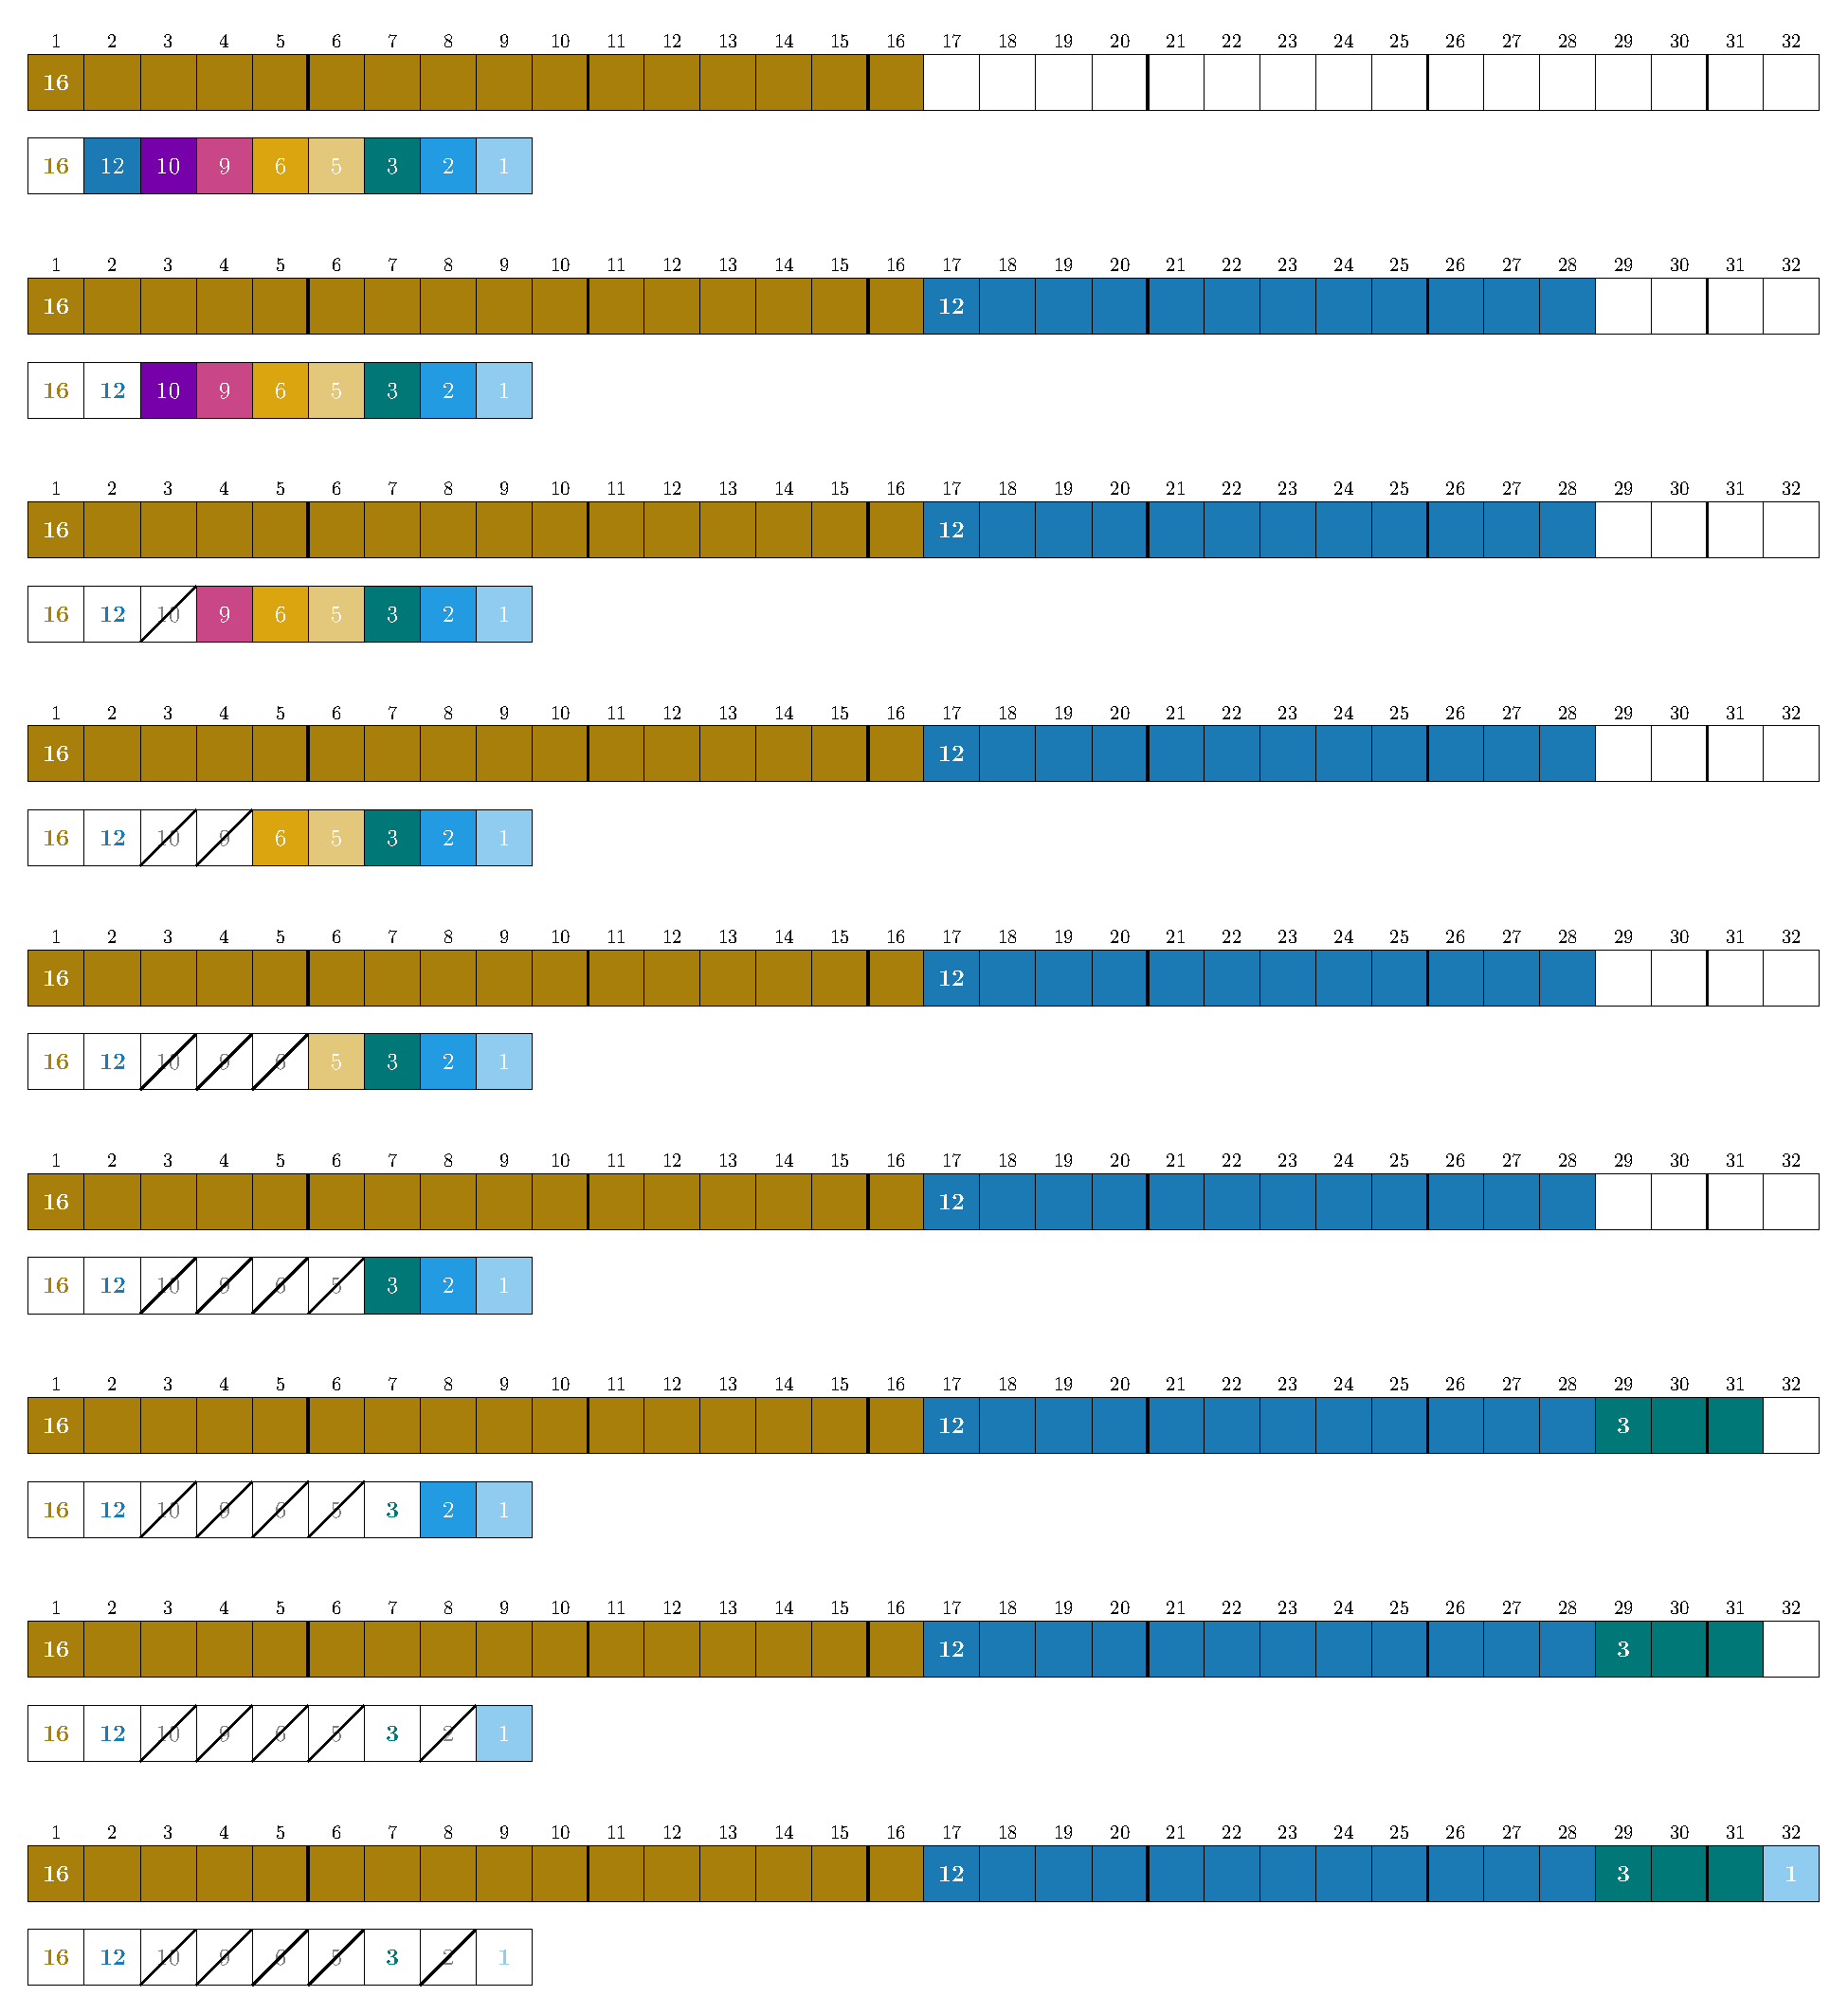
\includegraphics[width=0.6\linewidth]{ex1-9-GS.pdf}
    \caption{Solution de l'instance intermédiaire de type 1.}
  \end{figure}

\begin{exercice}{}
    Appliquer l'algorithme glouton sur une \instance{2}.
  \end{exercice}

  \begin{figure}[htbp]
    \centering
    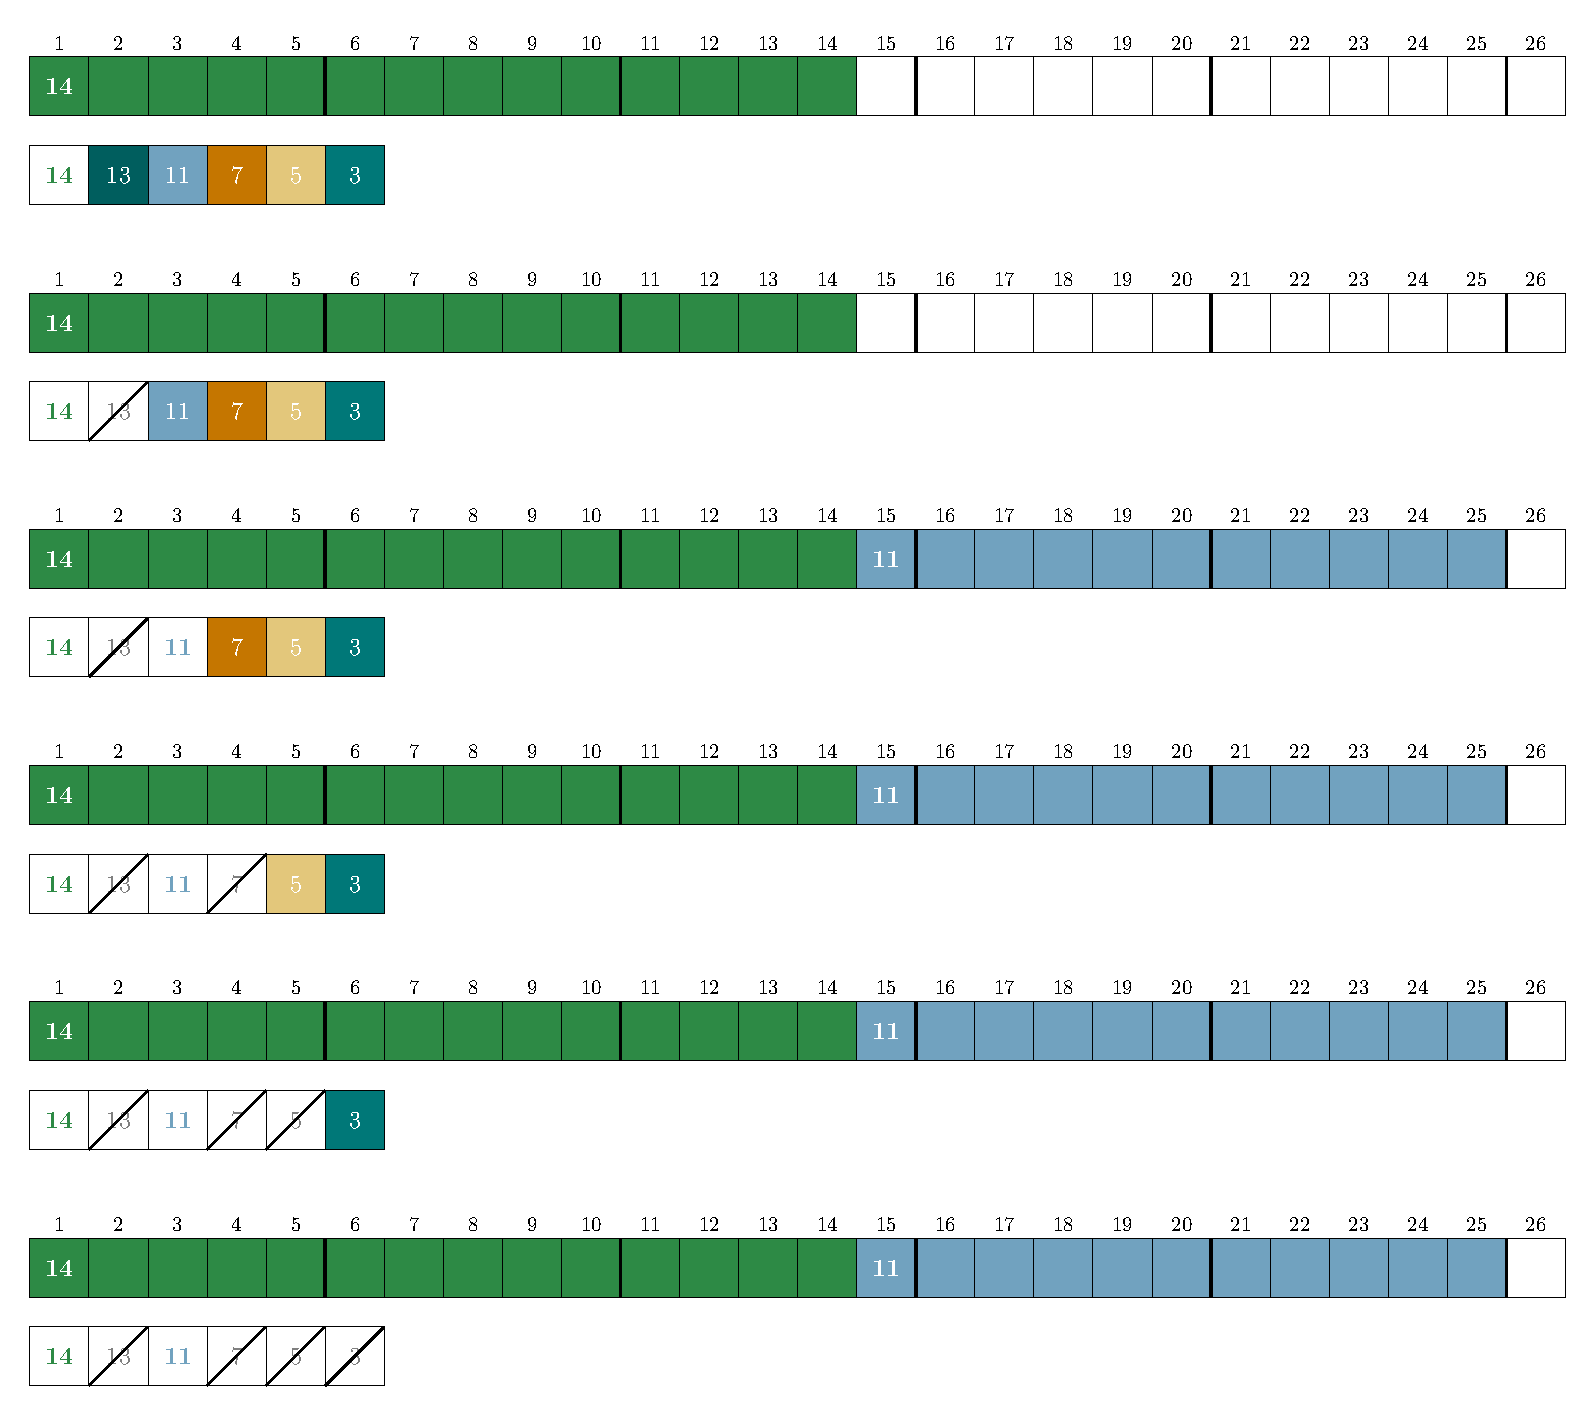
\includegraphics[width=0.6\linewidth]{ex2-6-GS.pdf}
    \caption{Solution de l'instance facile de type 2.}
  \end{figure}

  \begin{figure}[htbp]
    \centering
    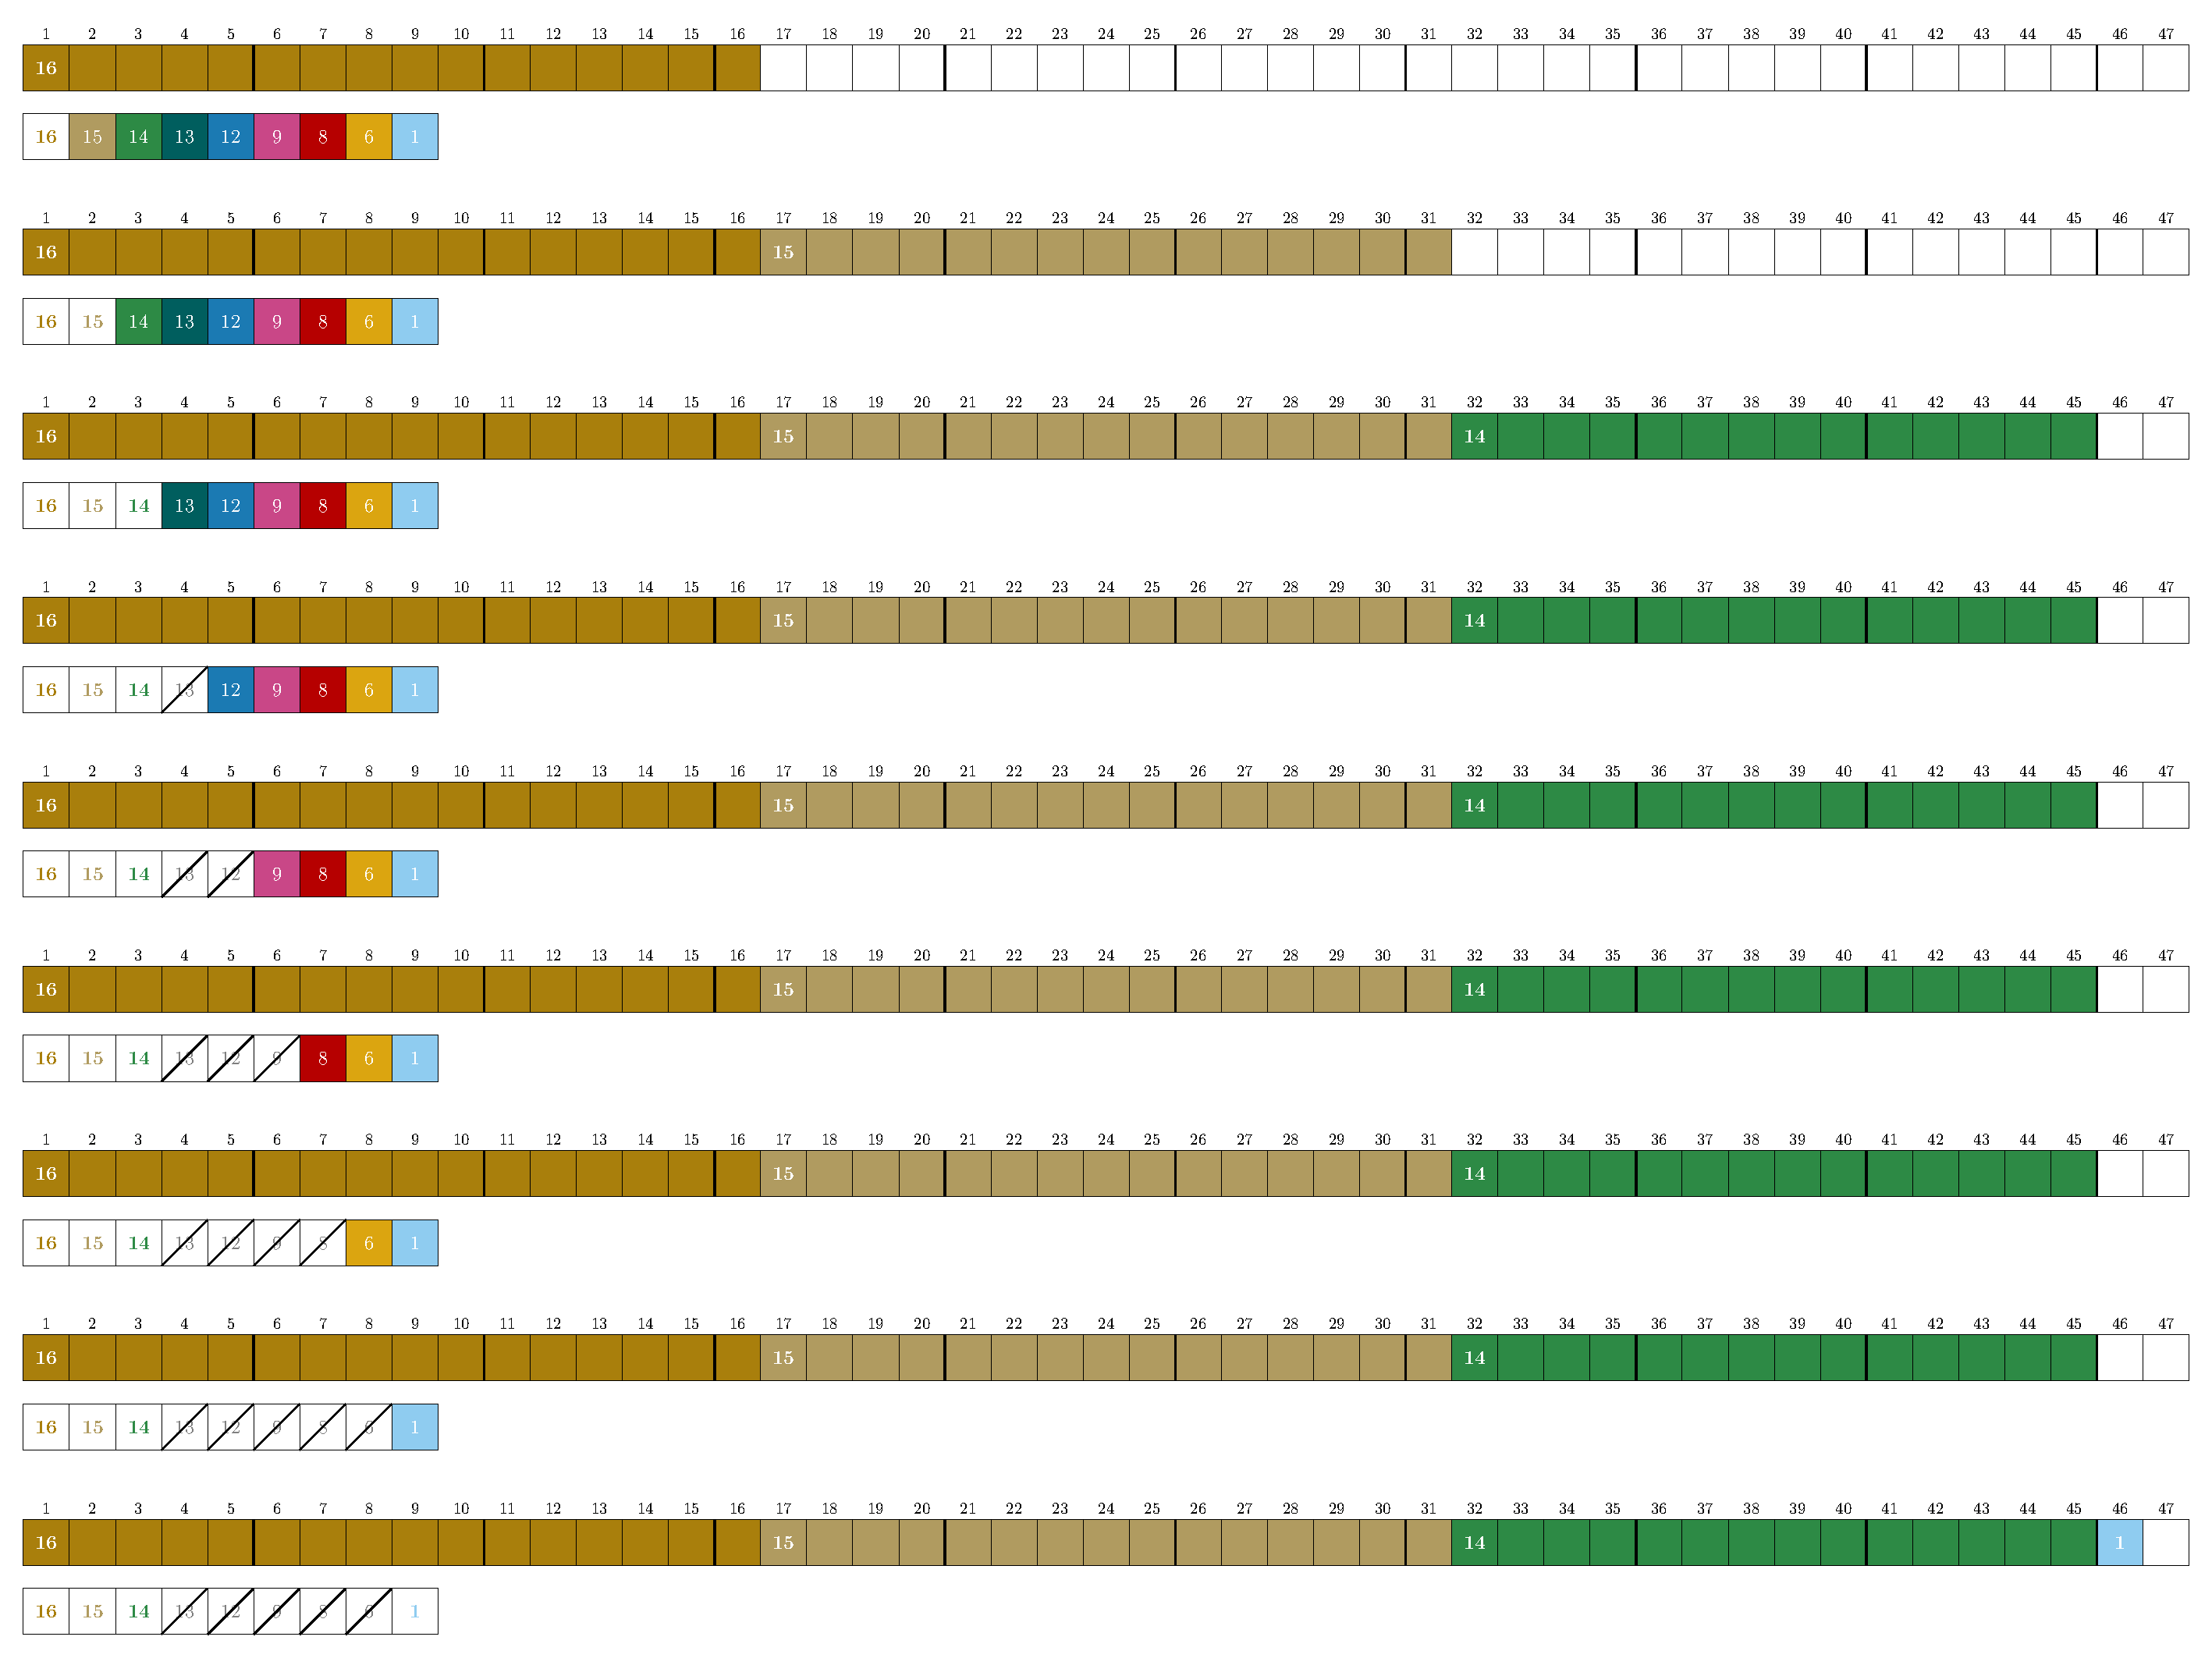
\includegraphics[width=0.6\linewidth]{ex2-9-GS.pdf}
    \caption{Solution de l'instance intermédiaire de type 2.}
  \end{figure}


  \begin{algorithme}{Algorithme glouton répété}
     \label{algo:mtgs}
    Répéter jusqu'à ce que le sac soit rempli ou contienne tous les objets :
    \begin{itemize}
    \item appliquer l'algorithme glouton ;
    \item éliminer le plus grand objet.
    \end{itemize}
  \end{algorithme}

  \begin{exercice}{}
    Appliquer l'algorithme glouton répété sur une \instance{2}.
  \end{exercice}

 \begin{figure}[htbp]
    \centering
    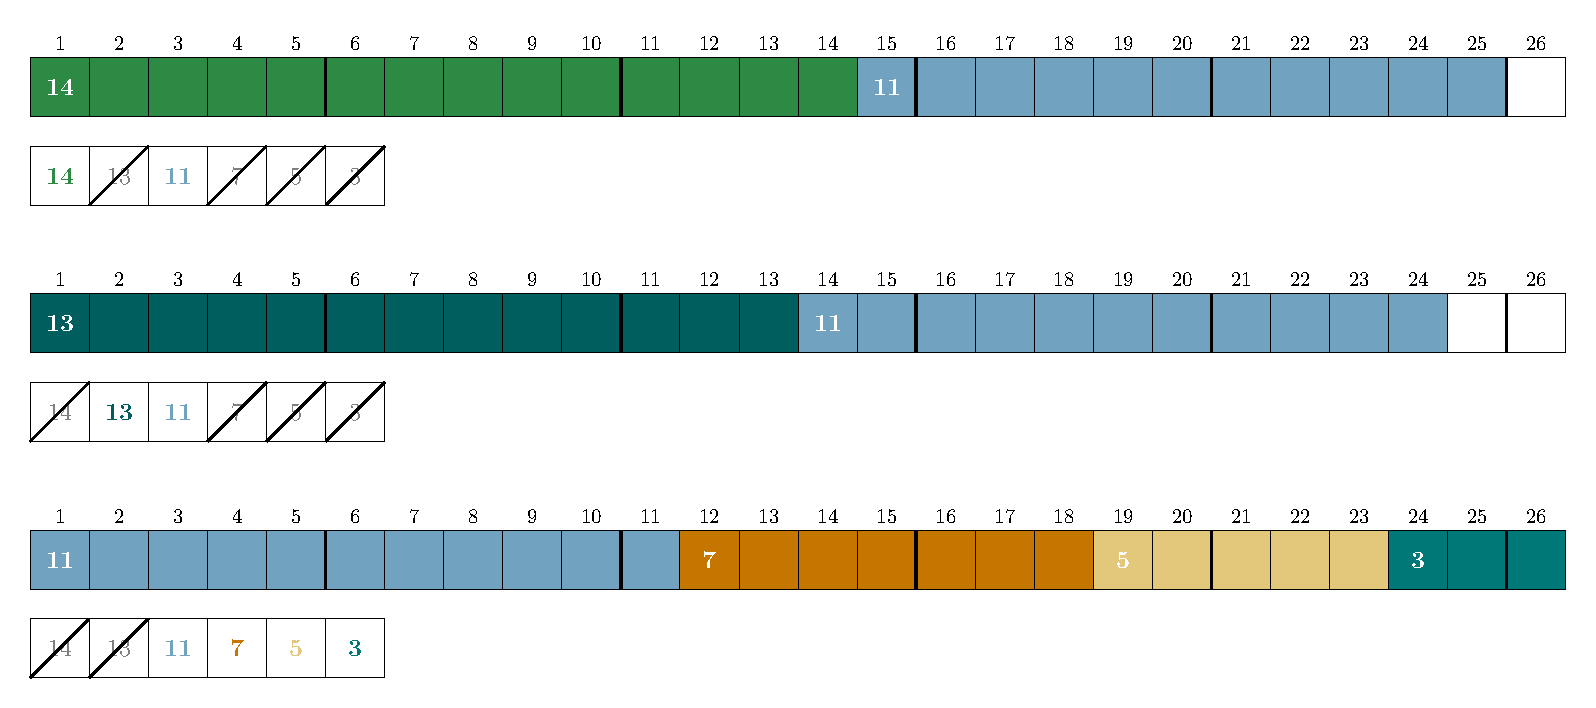
\includegraphics[width=0.6\linewidth]{ex2-6-MTGS.pdf}
    \caption{Solution de l'instance facile de type 2.}
  \end{figure}

  \begin{figure}[htbp]
    \centering
    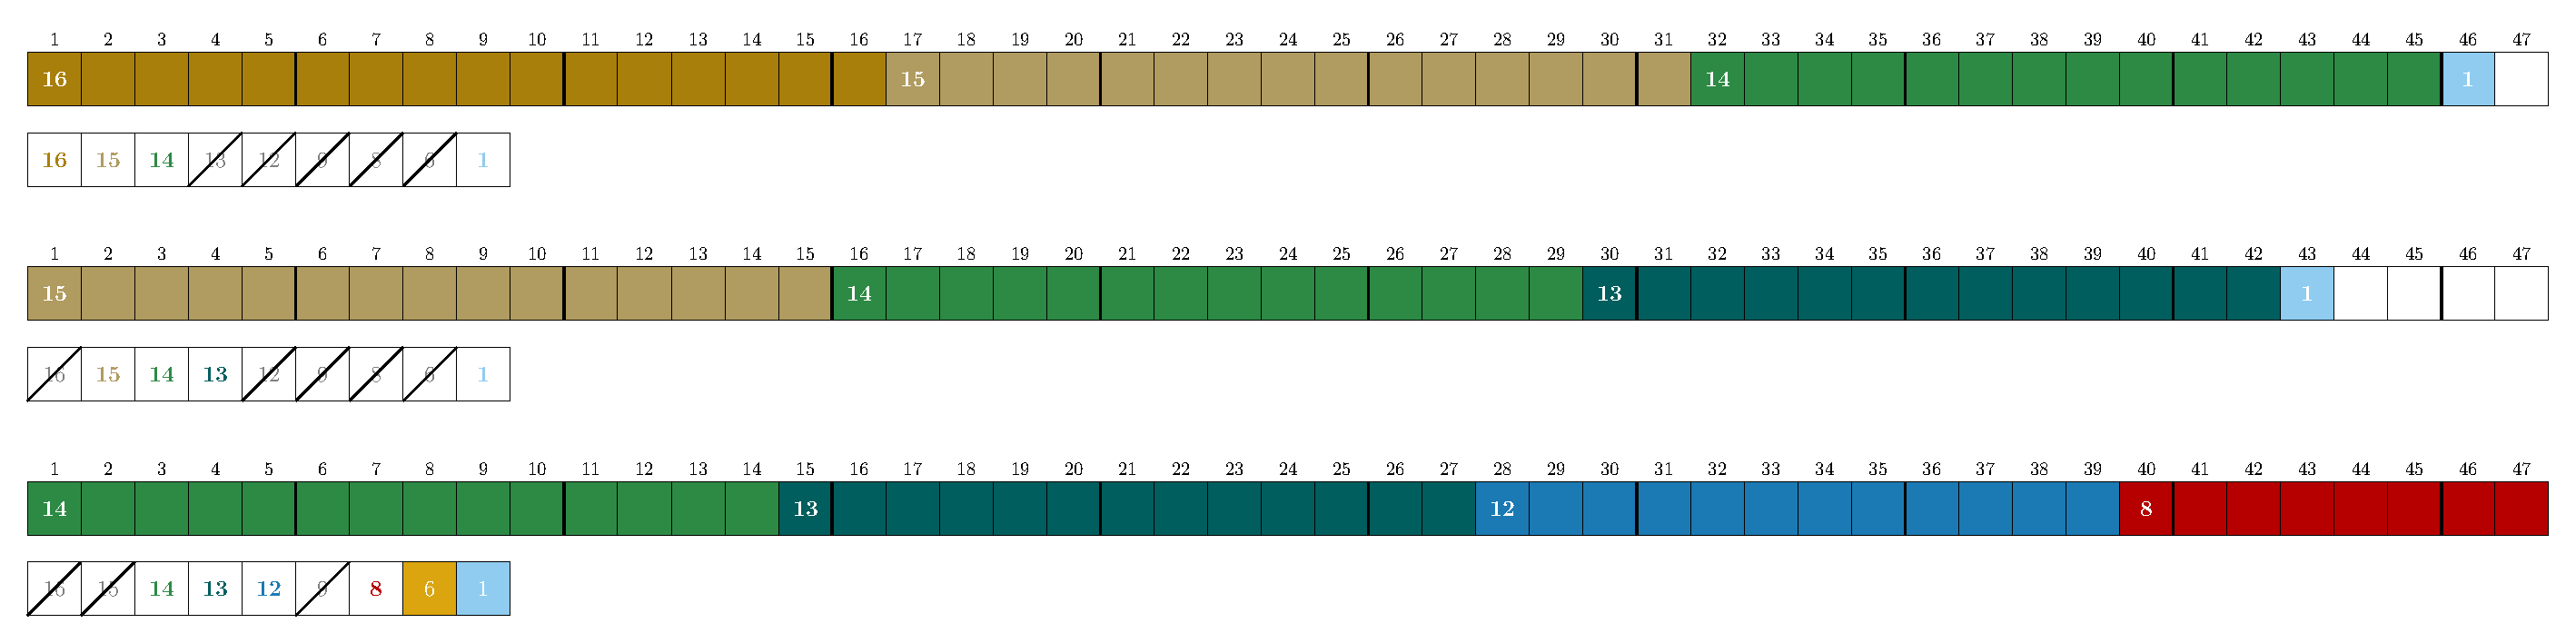
\includegraphics[width=0.6\linewidth]{ex2-9-MTGS.pdf}
    \caption{Solution de l'instance intermédiaire de type 2.}
  \end{figure}


   \begin{exercice}{}
    \label{ex:ex4}
    Appliquer l'algorithme glouton répété sur une \instance{3}
  \end{exercice}

 \begin{figure}[htbp]
    \centering
    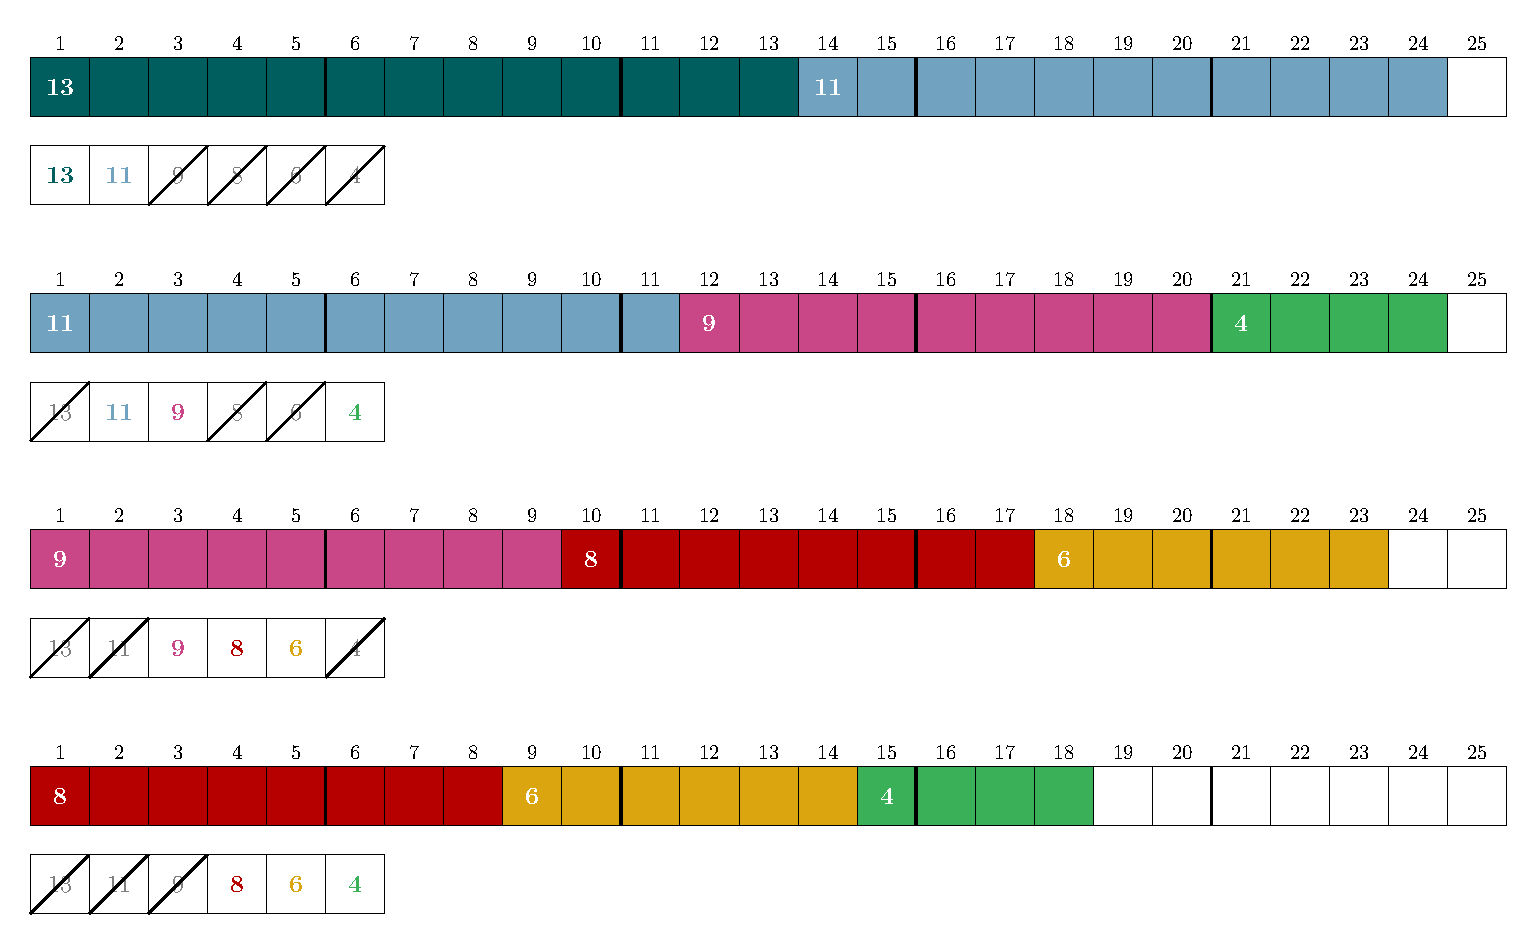
\includegraphics[width=0.6\linewidth]{ex3-6-MTGS.pdf}
    \caption{Solution de l'instance facile de type 3.}
  \end{figure}

  \begin{figure}[htbp]
    \centering
    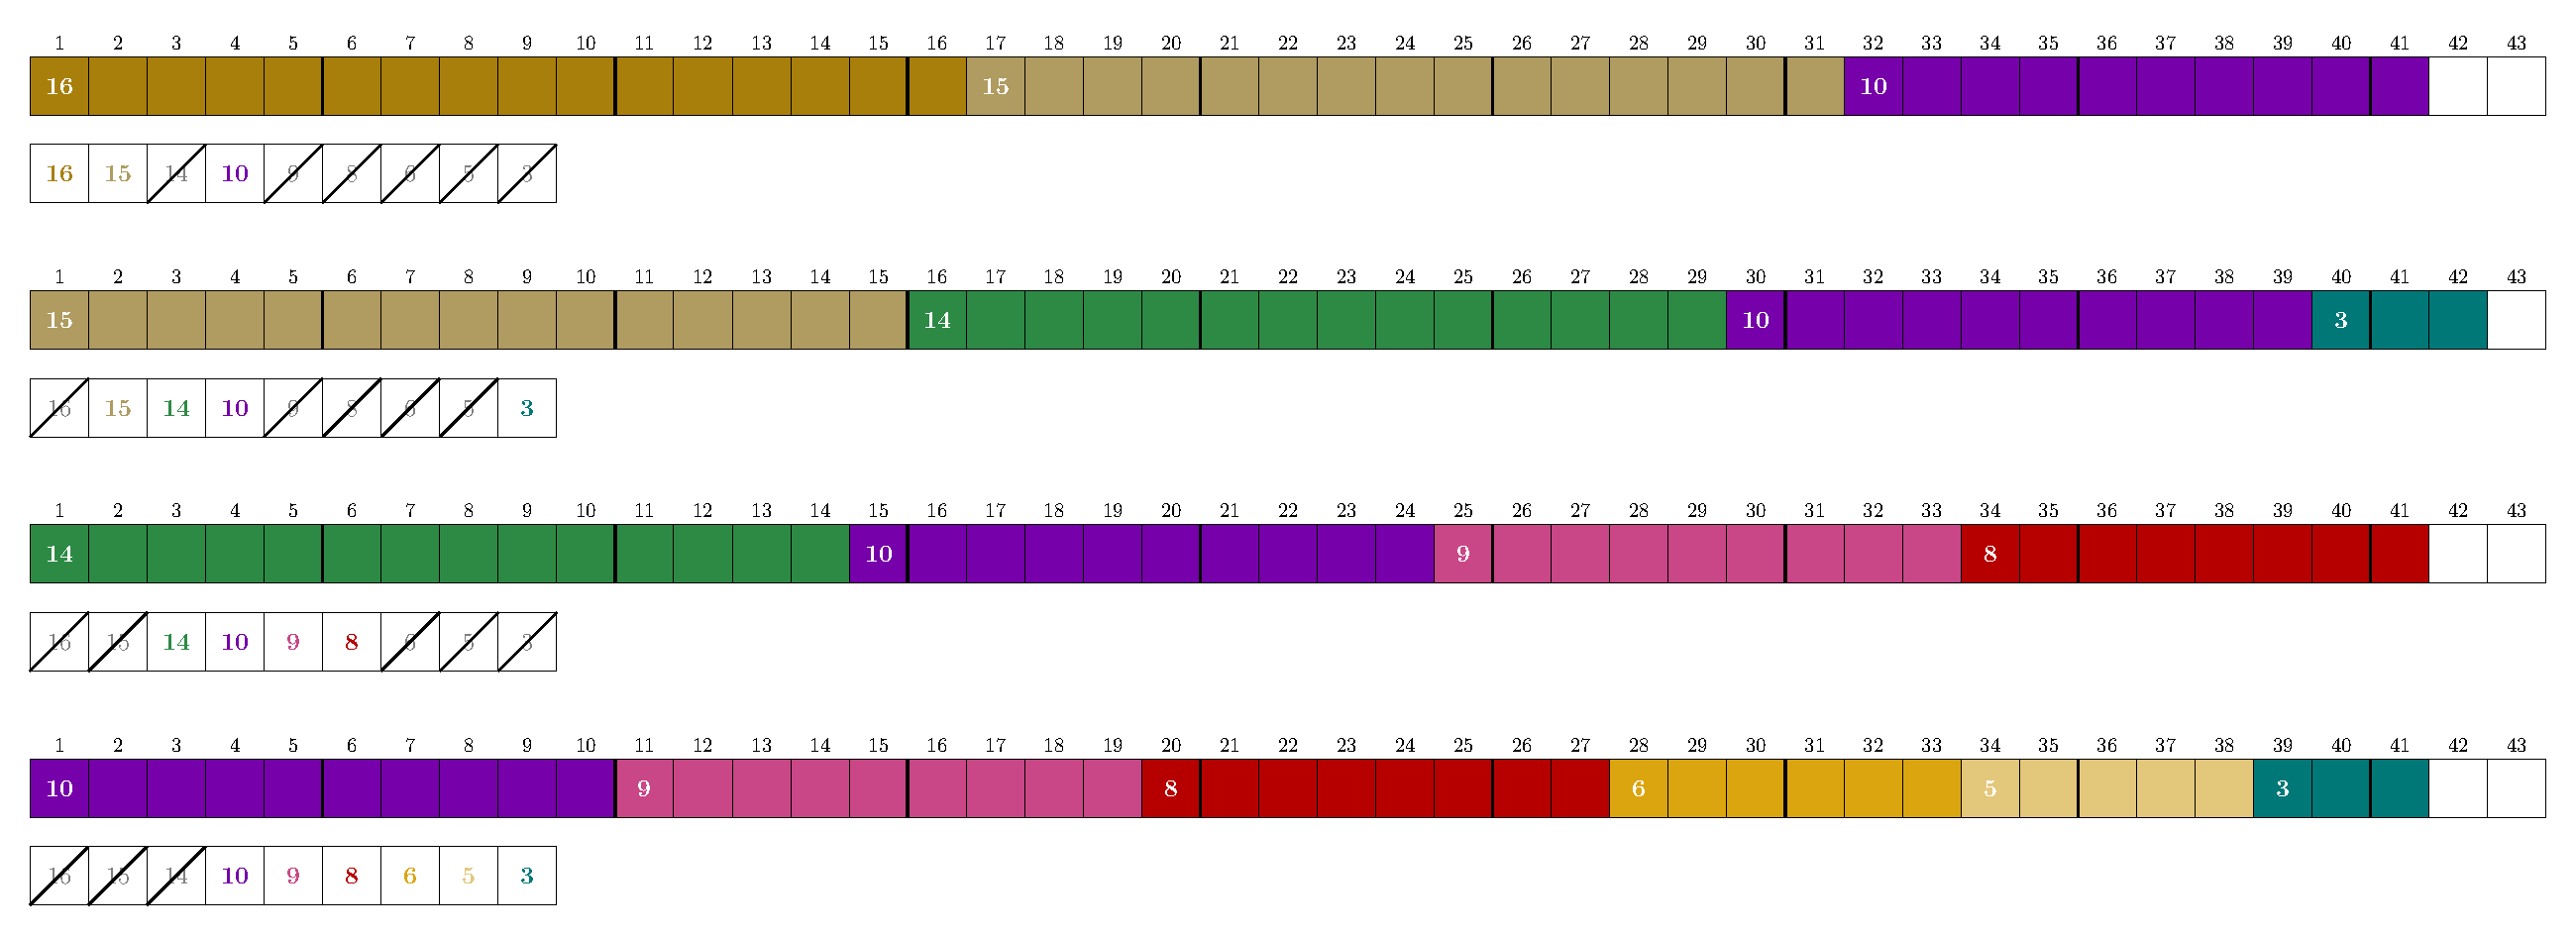
\includegraphics[width=0.6\linewidth]{ex3-9-MTGS.pdf}
    \caption{Solution de l'instance intermédiaire de type 3.}
  \end{figure}


  \section{Programmation dynamique}



  \begin{algorithme}{Algorithme de programmation dynamique}
    \begin{itemize}
    \item Déterminer la capacité du sac.
    \item Trier les objets par ordre décroissant.
    \item  Répéter tant qu'il reste des objets et que le sac n'est pas rempli (la dernière case n'est pas marquée) :
      \begin{itemize}
      \item répéter pour chaque case marquée en partant de la dernière :
      \begin{itemize}
      \item déterminer la case atteinte en rangeant l'objet immédiatement après la case marquée (utiliser l'objet comme règle).
      \item Si la case atteinte n'est pas marquée, placer un marqueur de l'objet.
      \end{itemize}
      \end{itemize}
    \end{itemize}
  \end{algorithme}


   \begin{exercice}{}
    \label{ex:ex5}
    Appliquer la programmation dynamique sur une \instance{3}.
  \end{exercice}

\begin{verbatim}
Inf  0  0  0  0  0  0  0  0  0  0  0  0  1  0  0  0  0  0  0  0  0  0  0  0  0
Inf  0  0  0  0  0  0  0  0  0  0  2  0  1  0  0  0  0  0  0  0  0  0  0  2  0
Inf  0  0  0  0  0  0  0  0  3  0  2  0  1  0  0  0  0  0  0  3  0  3  0  2  0
Inf  0  0  0  0  0  0  0  4  3  0  2  0  1  0  0  0  4  0  4  3  4  3  0  2  0
Inf  0  0  0  0  0  5  0  4  3  0  2  0  1  5  5  0  4  0  4  3  4  3  5  2  5
\end{verbatim}
\begin{figure}[htbp]
  \centering

    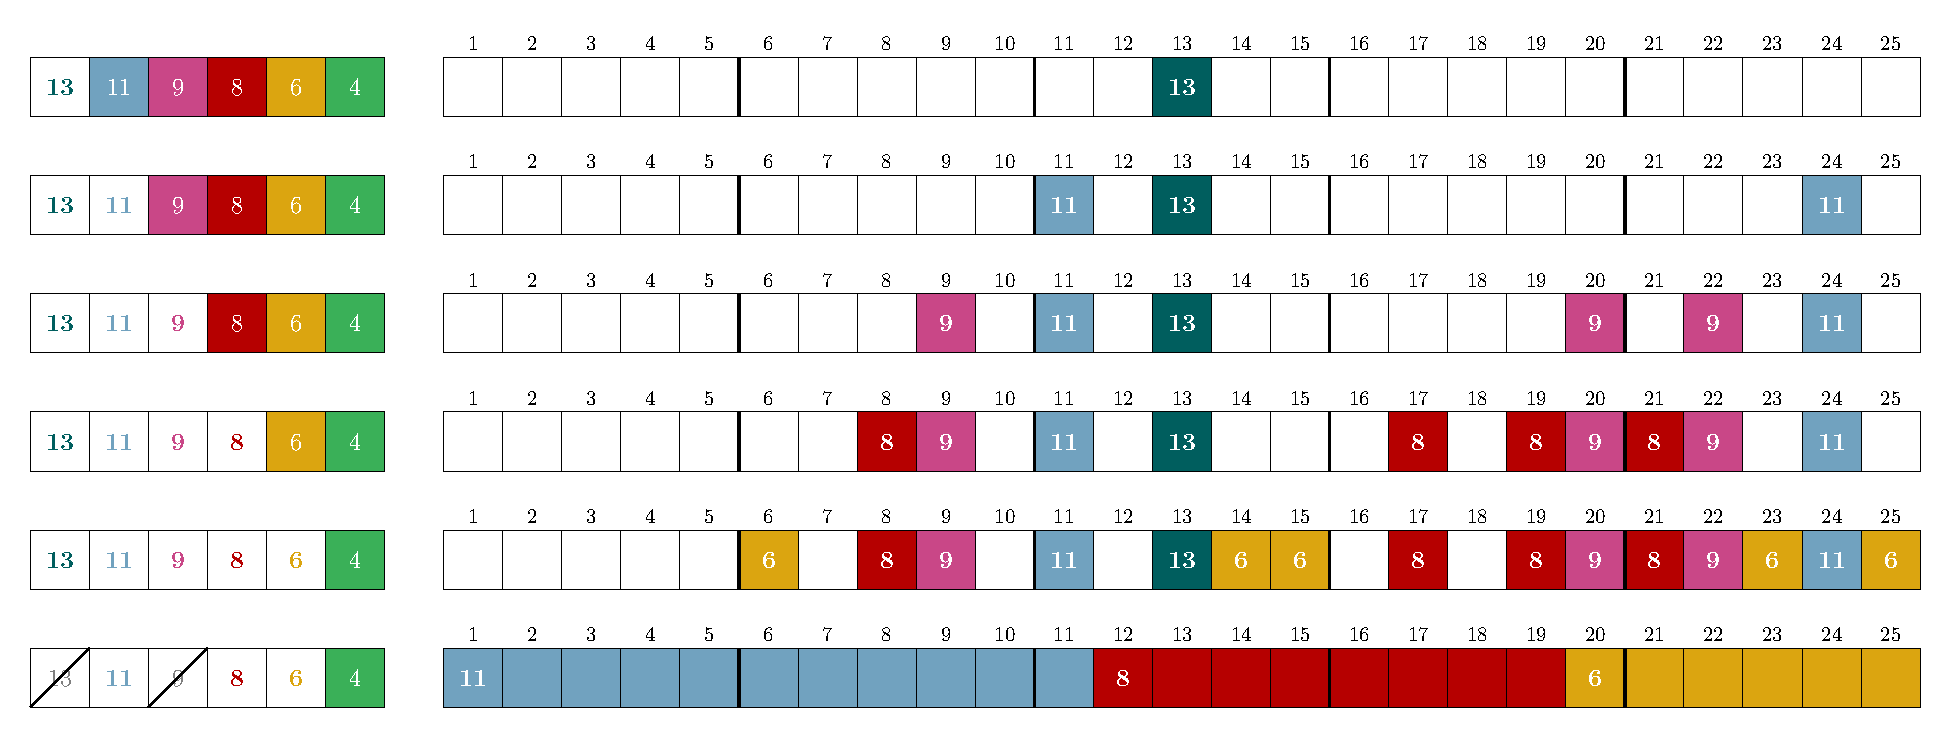
\includegraphics[width=0.6\linewidth]{ex3-6-DP.pdf}
    \caption{Solution de l'instance facile de type 3.}
  \end{figure}

\begin{verbatim}
 [1] Inf   0   0   0   0   0   0   0   0   0   0   0   0   0   0   0   1   0   0
[20]   0   0   0   0   0   0   0   0   0   0   0   0   0   0   0   0   0   0   0
[39]   0   0   0   0   0   0
 [1] Inf   0   0   0   0   0   0   0   0   0   0   0   0   0   0   2   1   0   0
[20]   0   0   0   0   0   0   0   0   0   0   0   0   2   0   0   0   0   0   0
[39]   0   0   0   0   0   0
 [1] Inf   0   0   0   0   0   0   0   0   0   0   0   0   0   3   2   1   0   0
[20]   0   0   0   0   0   0   0   0   0   0   3   3   2   0   0   0   0   0   0
[39]   0   0   0   0   0   0
 [1] Inf   0   0   0   0   0   0   0   0   0   4   0   0   0   3   2   1   0   0
[20]   0   0   0   0   0   4   4   4   0   0   3   3   2   0   0   0   0   0   0
[39]   0   4   4   4   0   0
 [1] Inf   0   0   0   0   0   0   0   0   5   4   0   0   0   3   2   1   0   0
[20]   5   0   0   0   5   4   4   4   0   0   3   3   2   0   5   5   5   0   0
[39]   5   4   4   4   0   0
 [1] Inf   0   0   0   0   0   0   0   6   5   4   0   0   0   3   2   1   6   6
[20]   5   0   0   6   5   4   4   4   6   0   3   3   2   6   5   5   5   0   6
[39]   5   4   4   4   6   6
 [1] Inf   0   0   0   0   0   0   0   6   5   4   0   0   0   3   2   1   6   6
[20]   5   0   0   6   5   4   4   4   6   0   3   3   2   6   5   5   5   0   6
[39]   5   4   4   4   6   6
\end{verbatim}
  \begin{figure}[htbp]
    \centering
    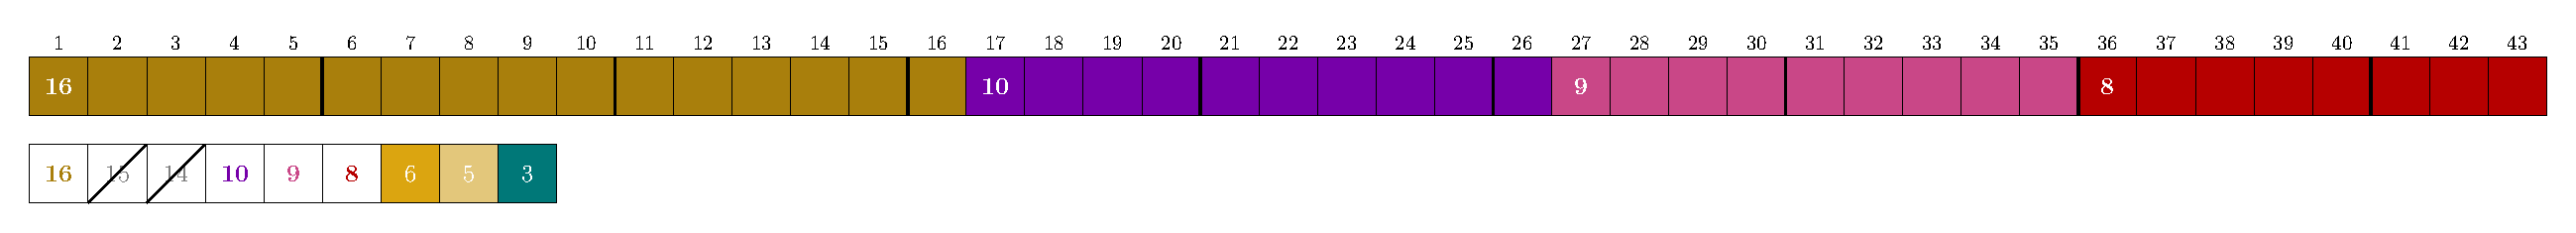
\includegraphics[width=0.6\linewidth]{ex3-9-DP.pdf}
    \caption{Solution de l'instance intermédiaire de type 3.}
  \end{figure}


  \begin{exercice}{}
    Appliquer la programmation dynamique sur une \instance{4}
  \end{exercice}

\begin{verbatim}
 [1] Inf   0   0   0   0   0   0   0   0   0   0   0   0   0   0   0   1   0   0
[20]   0   0   0   0   0   0
 [1] Inf   0   0   0   0   0   0   0   0   0   0   0   0   0   0   2   1   0   0
[20]   0   0   0   0   0   0
 [1] Inf   0   0   0   0   0   0   0   0   0   0   3   0   0   0   2   1   0   0
[20]   0   0   0   0   0   0
 [1] Inf   0   0   0   4   0   0   0   0   0   0   3   0   0   0   2   1   0   0
[20]   4   4   0   0   0   0
 [1] Inf   0   5   0   4   0   5   0   0   0   0   3   0   5   0   2   1   5   5
[20]   4   4   5   5   0   0
 [1] Inf   6   5   6   4   6   5   6   0   0   0   3   6   5   6   2   1   5   5
[20]   4   4   5   5   6   0
 [1] Inf   6   5   6   4   6   5   6   0   0   0   3   6   5   6   2   1   5   5
[20]   4   4   5   5   6   0
\end{verbatim}
    \begin{figure}[htbp]
    \centering
    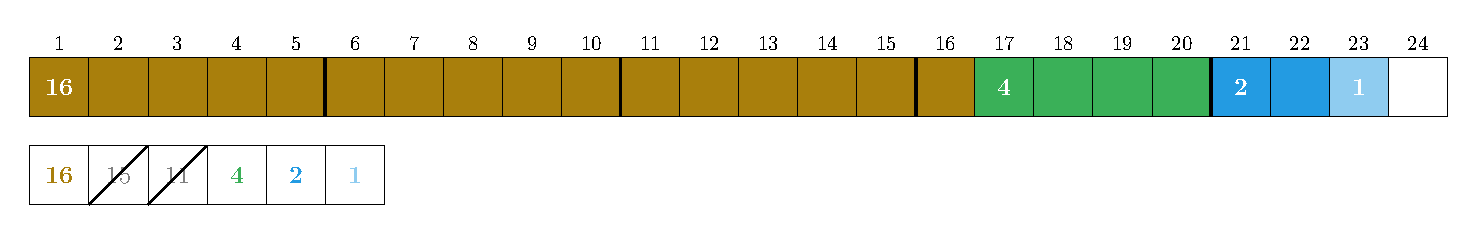
\includegraphics[width=0.6\linewidth]{ex4-6-DP.pdf}
    \caption{Solution de l'instance facile de type 4.}
  \end{figure}

\begin{verbatim}
 [1] Inf   0   0   0   0   0   0   0   0   0   0   0   0   0   0   0   0   0   1
[20]   0   0   0   0   0   0   0   0   0   0   0   0   0   0   0   0   0   0   0
 [1] Inf   0   0   0   0   0   0   0   0   0   0   0   0   0   0   2   0   0   1
[20]   0   0   0   0   0   0   0   0   0   0   0   0   0   0   2   0   0   0   0
 [1] Inf   0   0   0   0   0   0   0   0   0   0   0   0   3   0   2   0   0   1
[20]   0   0   0   0   0   0   0   0   0   3   0   0   3   0   2   0   0   0   0
 [1] Inf   0   0   0   0   0   0   0   0   0   4   0   0   3   0   2   0   0   1
[20]   0   0   0   0   4   0   4   0   0   3   0   0   3   0   2   0   0   0   0
 [1] Inf   0   0   0   0   0   0   0   5   0   4   0   0   3   0   2   0   0   1
[20]   0   0   5   0   4   0   4   5   0   3   0   0   3   0   2   0   0   5   0
 [1] Inf   0   0   0   0   6   0   0   5   0   4   0   0   3   0   2   0   0   1
[20]   0   6   5   0   4   0   4   5   0   3   0   6   3   0   2   0   0   5   0
 [1] Inf   0   0   7   0   6   0   0   5   0   4   7   0   3   0   2   7   0   1
[20]   0   6   5   0   4   7   4   5   0   3   7   6   3   0   2   7   0   5   0
 [1] Inf   0   8   7   0   6   0   8   5   0   4   7   8   3   0   2   7   8   1
[20]   0   6   5   8   4   7   4   5   8   3   7   6   3   8   2   7   8   5   0
 [1] Inf   0   8   7   0   6   0   8   5   0   4   7   8   3   0   2   7   8   1
[20]   0   6   5   8   4   7   4   5   8   3   7   6   3   8   2   7   8   5   0
\end{verbatim}
  \begin{figure}[htbp]
    \centering
    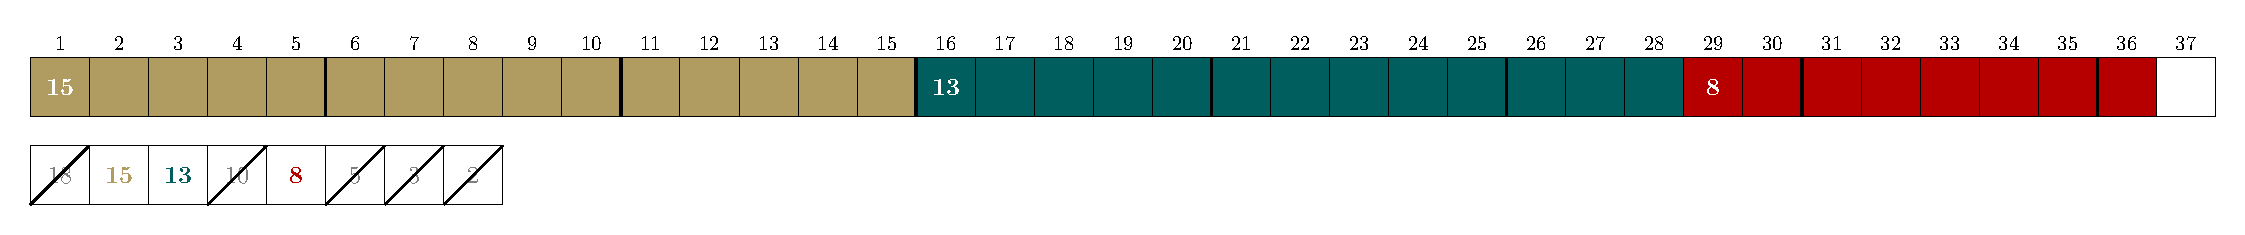
\includegraphics[width=0.6\linewidth]{ex4-8-DP.pdf}
    \caption{Solution de l'instance intermédiaire de type 4.}
  \end{figure}



  \section{Tester et Générer}

  \begin{algorithme}{Algorithme Tester-et-Générer}
    \begin{itemize}
    \item Déterminer la capacité.
    \item Trier les objets par ordre décroissant.
    \item  Descente : Répéter tant que le dernier objet n'est pas dans le sac :
      \begin{itemize}
      \item Répéter pour chaque objet :
        \begin{itemize}
        \item ranger l'objet dans le sac si la capacité le permet.
        \end{itemize}
      \item Si le sac est rempli, arrêter l'algorithme.
      \item Sinon, effectuer un retour arrière simple : retirer le plus petit objet du sac.
        \end{itemize}
      \item Retour arrière sautée quand le plus petit objet du deck est dans le sac.
      \begin{itemize}
      \item Retirer les objets du sac trouver jusqu'à ce que vous trouviez le plus petit objet que vous n'avez pas pu faire rentrer.


      \item Sinon éliminer l'objet.
      \end{itemize}
    % \item  Répéter tant qu'il reste des objets et que le sac n'est pas rempli (la dernière case n'est pas marquée) :
    %   \begin{itemize}
    %   \item répéter pour chaque case marquée en partant de la dernière :
    %   \begin{itemize}
    %   \item déterminer la case atteinte en rangeant l'objet immédiatement après la case marquée (utiliser l'objet comme règle).
    %   \item Si la case atteinte n'est pas marquée, placer un marqueur de l'objet.
    %   \end{itemize}
    %   \end{itemize}
    \end{itemize}
  \end{algorithme}



  \begin{exercice}{}
    Appliquer Tester-et-Générer sur une \instance{3}.
  \end{exercice}

\begin{figure}[htbp]
    \centering
    
\includegraphics[width=0.6\linewidth]{ex4-6-TG.pdf}
    \caption{Solution de l'instance facile de l'exercice~\ref{ex:ex4}}
  \end{figure}

  \begin{figure}[htbp]
    \centering
    % \includegraphics[width=0.6\linewidth]{ex4-8-TG.pdf}
    \caption{Solution de l'instance intermédiaire de l'exercice \ref{ex:ex4}}
  \end{figure}

  \begin{exercice}{}
    Appliquer Tester-et-Générer sur une \instance{4}.
  \end{exercice}


  \section{Problèmes connexes}

  % \subsection{Subset Sum Problem}
  % \cite{SSP}

  % \subsection{Ordonnancement}
  % \cite{MS}
  % \cite{Korf2013}

  % \subsection{Sac-à-dos}
  % \cite{KP}
  % \cite{MartelloToth1990}

  % \begin{tikzpicture}
  %   \filldraw [fill = bleuTN] (0, 2) rectangle (8, 3);
  %   \filldraw [fill = rouge] (8, 2) rectangle (14, 3);

  %   \draw [<->, very thick, exCol] (7, 3.25) -- (8, 3.25) node [right] {Ordonnancement};

  %   \filldraw [fill = rouge] (0, 0) rectangle (6, 1);
  %   \filldraw [fill = bleuTN] (6, 0) rectangle (14, 1);

  %   \draw [<->, very thick, orange] (7, -0.25) -- (6, -0.25) node [left] {Sac-à-dos};

  %   \draw [<->, very thick, violet] (6.5, 1.5) -- (7.5, 1.5) node [right] {Partition};

  %   \draw [dashed, very thick] (7, -0.75) -- (7, 3.75) node [above] {C};
  % \end{tikzpicture}




  \begin{algorithme}{}
    test
  \end{algorithme}


  \begin{plusloin}{}
    test
  \end{plusloin}

  \bibliographystyle{plain}
  \bibliography{poly}
\end{document}
